\chapter{Evaluation}
\label{chapter:evaluation}


The most obvious aspect to improve in the program is usability. Currently the tool requires manual fetching of the input data in json format from the client company's system by adjusting the API address url to get the data from a specific date range. This data has to be then saved to a file and put to the program folder. 

The program has to be run from command line or alternatively by double clicking on the .jar file if the operating system supports this behaviour. In the latter case, the program does not show any progress information to the user.

\section{Results}
the program was run on a PC running Windows 7 with an Intel 3,4 GHz quad core CPU and 16 GB of 1,6 GHz RAM. The Java version used was 1.8.0\_66. 

Running time depends greatly on whether the distance information has been cached or if it has to be fetched from MapQuest's routing API. A sample run with 574 job targets split between 42 technicians and an iteration count of 256 showed that without any cached results, the program took 57.7 seconds to run, and on a second go with cached distance data, the program took 9.2 seconds to complete. Profiling the program indicates that most of this time is spent in the library solving functions. About 15 \% of time was spent serialising and de-serialising the cached route data and the rest was spent on the actual problem solving.

Because the actual routes are very short (71 \% of routes consist of only one job target, 21 \% of routes have two targets, 7 \% have three and mere 1 \% of routes include 4 targets), the inherent benefits of the Jsprit's implementation of the ruin and recreate method are not apparent. A simple savings algorithm probably could reach almost similar solution quality. In the context of this project this does not matter, however, as an already existing library provided the advanced functionality with no extra cost. 


The number of iterations used for the solving did not affect the results much. The total time cost of all the routes was used as the measurement of solution quality. As figure~\ref{fig:iterations} shows, the benefit of the ruin and recreate algorithm is minimal. When only the driving time is observed, the initial solution with 0 iterations is only 3.1 \% slower than the solution reached with 4096 iterations. When the working time at targets is also taken into account, the difference is slightly less than 1 \%. The computational cost of a single iteration is constant. Doubling the number of iterations also doubles the solving time. In figure~\ref{fig:iterations} the solving time is doubled on every step. It can be seen that the benefits of increasing the number of iterations in the algorithm gradually lower until they become non-existent at 2048 iterations. 

\begin{figure}[h]
  \begin{center}
    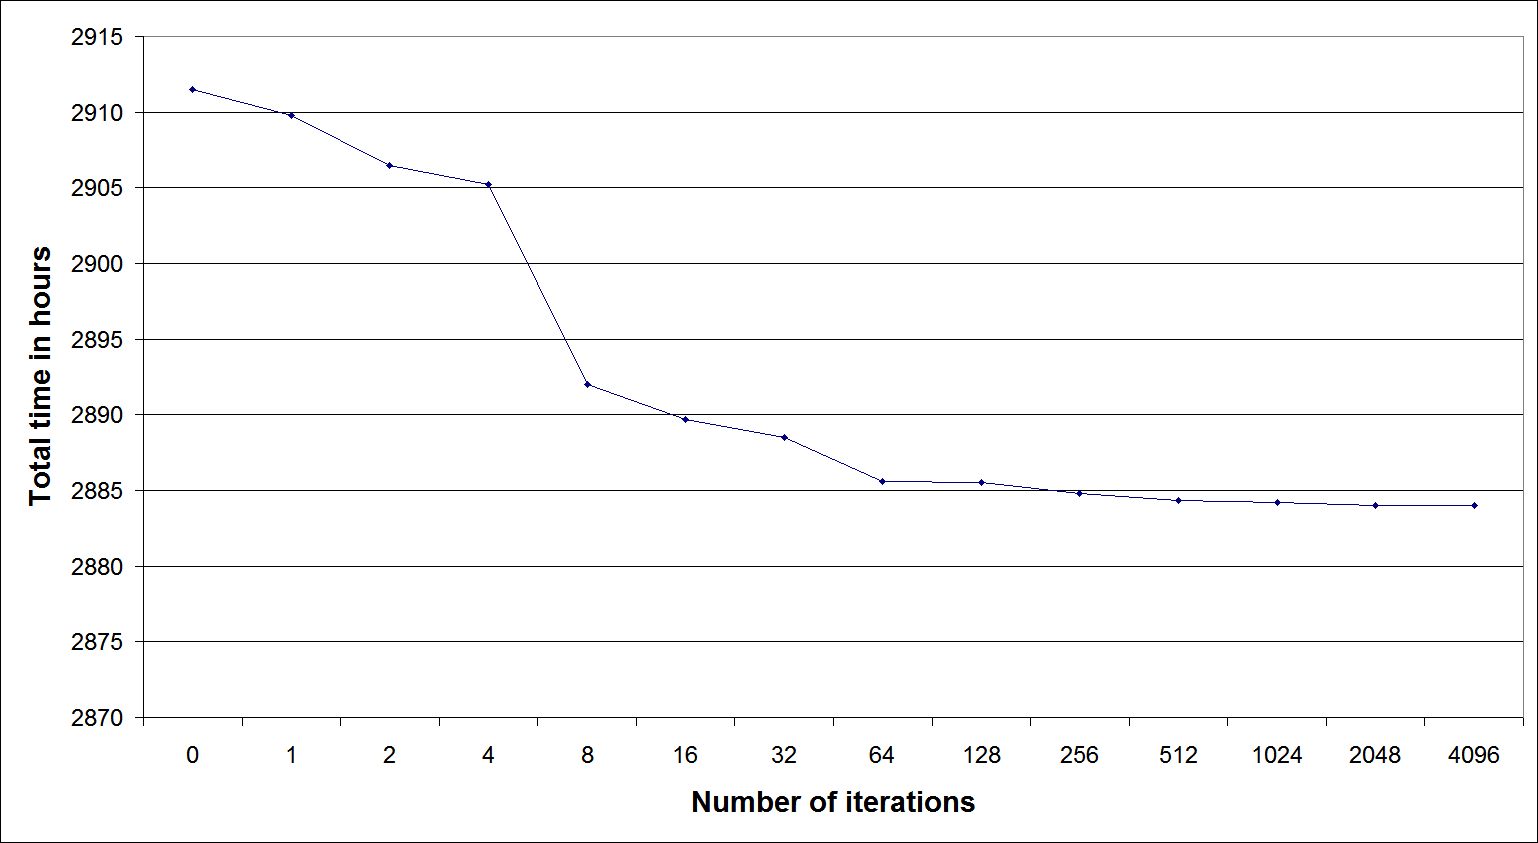
\includegraphics[width=\textwidth]{images/iterations.png}
    \caption{The total driving time cost of all routes with varying numbers of iterations. With 0 iterations the solution is just the initial solution created by jsprit.}
    \label{fig:iterations}
  \end{center}
\end{figure} 

The small differences should not be downplayed, either. In this case, the difference between the very worst and the best solution translates to 27.5 hours. Saving that many hours per month can be a sizeable savings for a company. However, the difference between 4096 and 64 iterations is only 1,5 hours in total. Finding the optimal spot between performance and solution quality lies somewhere between those two values, in my opinion. 64 iterations is an operation fast enough that it practically does not break the user's workflow, while 4096 iterations causes a very noticeable delay. With the test data and cached location data, the total run time with 4096 iterations was 2 minutes and 26.7 seconds, while with 64 iterations it was 4.5 seconds.

If the routes were produced company-wide and then assigned to the technicians afterwards, the benefits of the algorithm would become more apparent. Currently there are about 10-25 job targets per technician during the one month planning period, leaving a relatively low number of possible combinations to try out. However, using the company-wide system would put more strain on the travelling cost matrix generation. Instead of multiple small all-to-all networks, there would be one big one, requiring additional optimisations to avoid having to make tens of thousands of queries to a routing API per solving.   




\section{Customer's perspective}

The customer was able to run the program and make it produce the expected output. The customer was overall pleased with the program's output and found that it could be used for planning routes. The quality of the routes was similar to that of routes produced by manual labour. This was determined by counting the number of days needed to handle a set of jobs.  

This program, a preliminary demo of what is possible to do, caused interest in the client company to continue the development the work planning procedures used in the company and automate them further. The next step would be optimising the way the job targets are assigned to the various technicians. This will likely provide much more optimal results, as inefficient allocation of jobs might make it impossible to do the routing process itself well. Automating the whole process would also grant the possibility of objectively comparing different approaches to work planning, as one method will provide a less travelling overhead than another and the results are immediately measureable.   

The biggest downside found by the client in the current program was that there can be quite a large gap in the earliest possible installation date between the jobs on a single route. This is because currently the program does not care about the earliest installation date except at results outputting. Aside from this issue, the client did not find problems with the program. A crude workaround solution is to simply use input data with more restricted date filtering. If only job targets aimed to be done within a certain week are included in the input, there cannot be large gaps between the earliest installation dates of targets in a route.

The customer also would have wanted ordering of the routes by dates. Currently the routes are displayed in random order as the routes can be assigned to any date. The scheduling should be designed so that routes that visit the same areas should be on subsequent days.



\section{Future development}

Probably the biggest room for development lies in usability. Using the program for a specific installer or automatically fetching the input data according to user preference would make the program's usage a lot more comfortable. The lack of user interface makes the program potentially confusing for a non-expert.


\subsection{Business logic}

Currently the program uses very rough estimates for determining the time required at a worksite. 1 hour per item and a fixed 15 minute overhead work fine for testing purposes, but more detailed information would provide better and more optimised routes. This would be a rather simple task that would be achievable with the usage of configuration files, for example. This would also make it relatively simple to make the program support new types of installation items and more specifically categorise building types.

The user could enter the average time requirements per installation item type based on past experience on worksites where the item has been installed. The effect of different house types and the floor number of the operation could be taken into account. Furthermore, the relative performance of technicians could be listed, allowing the scaling of the time requirement to get as accurate estimation as possible.

As the program provides only routes for the future, it does not take into account any potential setbacks, such as sick leaves, car malfunctions and so on. As the routes themselves outputted by the program do not have any specific date, but rather only an earliest possible date, it could be thought that a sick leave, for instance will only require postponing the routes in calendar.  

The client company's request for following the time windows more strictly is also a clear way to improve the results provided by the program. Considering that the jobs should start as soon as possible after the construction materials have been delivered to the worksite, the algorithm should try to group targets with near delivery dates onto same routes. Currently the algorithm can create routes such that the delivery of the installation materials of the earliest job is weeks before the delivery of the latest job, resulting in a scenario where the materials will lie unused at the worksite of the earlier job for weeks. This would lead to reduced customer satisfaction.

One way to address the aforementioned issue would be to assign a penalty to routes with a big variety in the earliest installation dates. This would result in the algorithm favouring routes where the jobs' earliest installation dates are grouped more tightly together. This would require implementing the aforementioned additional feature to the Jsprit library which might be a lot of work. 

Another way would be to group the installation jobs by their earliest installation dates. This would be easy to implement. However, it would be difficult to tell if a certain job would fit better in the next group, resulting in potentially unnecessarily suboptimal routes. This could be countered by running the algorithm multiple times and adjusting the date ranges of the groups between runs. Then the best routes could be picked from the results. However, this would require more complex results analysis due to jobs being found in multiple routes. 

\subsection{Output}
The results output is currently just textual representation with the routes and the routes' job locations indented for clarity. A proper visual representation of the routes and suggested dates for them would make benefitting the results much easier. The Jsprit library supports exporting the results in xml format already, so producing a custom machine-readable output is not necessary, unless using a simpler schema or some format other than xml is required.

Performance of the program could be improved by solving the separate technicians' VRPs in parallel. Considering how quick the actual solving process was, I did not see much point in implementing this kind of concurrency to the program. 

\subsection{Programming aspects}
The structure of the program would need refactoring, as it was developed for research purposes with a lot of trial and error. Though the codebase is very small, less than 1000 lines, restructuring and otherwise cleaning the code is necessary if this software is to be used in a bigger context.

The program's error handling capabilities are also very limited. Most errors cause the program to crash or produce bad or non-existent results without giving an understandable error message. This is not an issue for research use, but real world usage would definitely benefit from a more solid error handling. 

All testing on the program was done by hand. Automated testing would make future development a lot easier.


\section{Retrospective}

Overall, I feel like this project was a success. I reached the goals I had set beforehand and firmly believe that the future development of the program is not only possible, but would increase the amount of potential benefit in work planning.

The implementation process went fine without any unsolvable show stoppers which would have required doing workarounds for the desired outcome.  

With highly versatile libraries such as Jsprit, the main problems to tackle involve adapting the business logic to the algorithm's framework.  